% Generated from saved defense family by make_defense.py.
\subsection{Paired pre-NMS defense timing}
\label{app:seg-laptop-defense}
After the two accepted CPU sessions, a separate prospective protocol fixes two interventions: cap candidates before NMS at 300, or cap retained outputs at 50. Each comparison uses the identical frozen attacked tensor in both arms and a newly measured, interleaved baseline (candidate cap 30000, output cap 300). The device, model, fixed NMS backend, resolution and carryover-balanced duplicate-label schedule follow the laptop method above. Each block has its own smoke and conditional full run, independent quality gate, SHA-bound source/input lock and app-affinity restoration. A temporary probe records the actual compiled-kernel input count outside timing and restores the original function before warmup and measurement.
\begin{table*}[t]\centering
\caption{Predetermined defense comparisons. Only the pre-NMS intervention reached full timing qualification. The failed output-cap smoke is retained and its full run was cancelled, without retry.}
\label{tab:seg-laptop-defense}
\begin{tabular}{lrrrr}\toprule
Intervention & Defended/baseline [95\% CI] & Baseline A/A MDE (\%) & Defended A/A MDE (\%) & Drift flags\\\midrule
Pre-NMS cap 300 & 0.526773 [0.507007, 0.548921] & 0.149061 & 0.314700 & 1/22 \\
Output cap 50 & Not qualified; full cancelled & --- & --- & 1/4 (smoke) \\
\bottomrule\end{tabular}\end{table*}
For the pre-NMS cap, total latency decreases by 47.322709\% [pointwise 95\% CI 45.107882, 49.299341]. The mean paired difference of image medians is -468.920147 ms [95\% CI -510.113507, -425.613187]. Each interval uses the registered 20000 image-bootstrap replicates; these intervals are not simultaneous family-wise intervals.
All 20 image log ratios have the same negative sign. The two-sided exact sign-flip calculation enumerates all $2^{20}$ assignments, giving $p=2/2^{20}$; Holm adjustment over the two registered comparisons gives $p_{\mathrm{Holm}}=4/2^{20}$. The unmeasured/failed output-cap comparison contributes a testing placeholder of one to preserve family size; that value is not a finding of no effect. Sign-flip inference assumes sign exchangeability under the null and does not create random-population sampling or additional image independence.
Observed kernel inputs fall from 1726--3744 to exactly 300 for every image. Retained masks change from a median of 270.5 (range 177--300) to 98 (84--118). Thus the intervention bounds kernel input but retains nonzero mask work; this total-pipeline contrast does not separately attribute savings to NMS and mask rendering. All raw spikes remain, including 50/1920 baseline and 29/1920 defended calls exceeding 1.5 times their image-specific median, each with process-CPU/wall below 0.75.
\begin{figure*}[t]\centering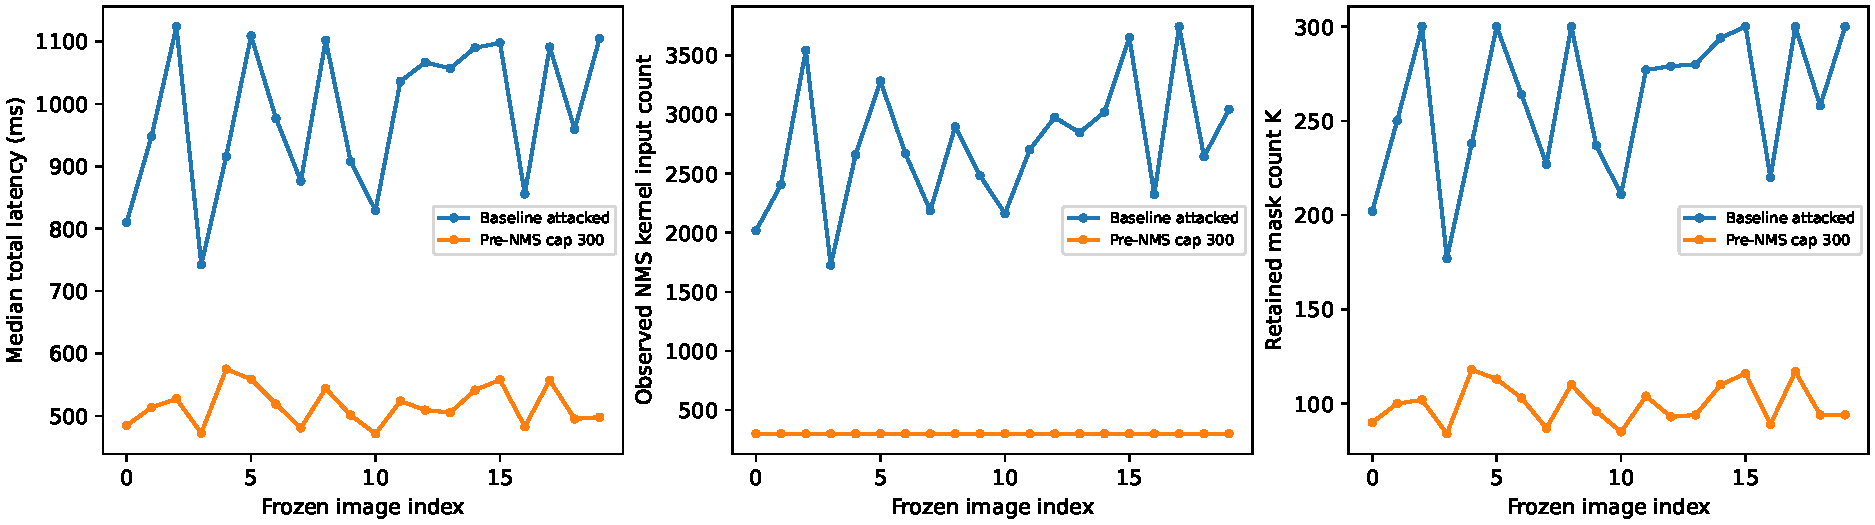
\includegraphics[width=.98\textwidth]{segmentation_extension/laptop_defense.pdf}\caption{Qualified pre-NMS intervention: per-image median total latency, observed compiled-NMS input count, and retained mask count. Counts and timing have separate axes and units.}\label{fig:seg-laptop-defense}\end{figure*}
The output-cap smoke had a forward-reference ratio of 1.0376245029873103 at its first image, exceeding the registered 3\% bound; its apparently lower timings remain diagnostic and are not used as a qualified defense estimate. Both blocks restored all 45 application processes. The study tests fixed saved perturbations, not an adaptive adversary trained against the cap. The earlier clean-accuracy evaluation used confidence 0.001 and letterboxing, unlike this confidence-0.25 square-tensor latency protocol; no jointly matched accuracy--latency curve or availability guarantee is inferred.
